\begin{center}
    \textbf{Geração 1000}
\end{center}

\begin{figure}[h]
    \centering
    \label{fig:geracao01}
    
    \begin{tabular}{rl}
        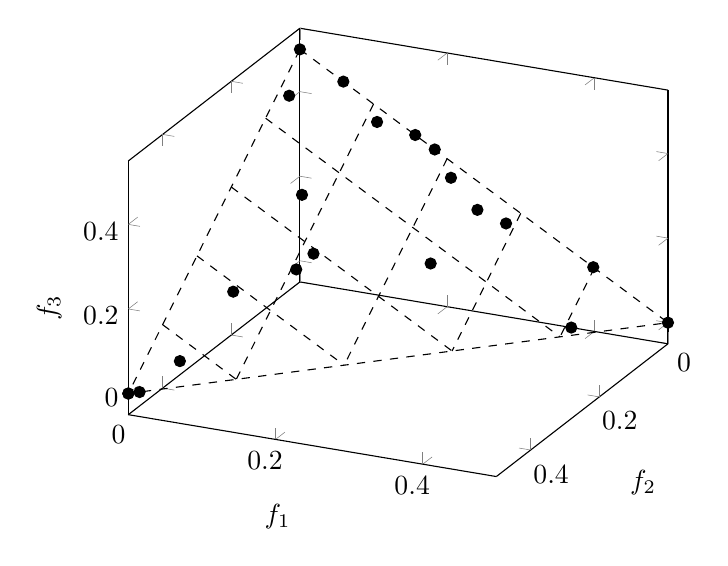
\begin{tikzpicture}[scale=1.0]
        	\begin{axis}[xlabel=$f_2$, ylabel=$f_1$, zlabel=$f_3$, view/h=115]
        		
    			\addplot3[style={dashed}]coordinates {
    			    (0., 0., 0.5) (0., 0.5, 0.) (0.5, 0., 0.) (0., 0., 0.5)
    			};
    			
    			\addplot3[style={dashed}]coordinates {(0., 0.1, 0.4) (0.4, 0.1, 0.)};
    			\addplot3[style={dashed}]coordinates {(0., 0.2, 0.3) (0.3, 0.2, 0.)};
    			\addplot3[style={dashed}]coordinates {(0., 0.3, 0.2) (0.2, 0.3, 0.)};
    			\addplot3[style={dashed}]coordinates {(0., 0.4, 0.1) (0.1, 0.4, 0.)};
    			
    			\addplot3[style={dashed}]coordinates {(0.4, 0., 0.1) (0.4, 0.1, 0.)};
    			\addplot3[style={dashed}]coordinates {(0.3, 0., 0.2) (0.3, 0.2, 0.)};
    			\addplot3[style={dashed}]coordinates {(0.2, 0., 0.3) (0.2, 0.3, 0.)};
    			\addplot3[style={dashed}]coordinates {(0.1, 0., 0.4) (0.1, 0.4, 0.)};
    			
    			\addplot3[only marks] coordinates {
            		(0.500000, 0.000000, 0.000000) (0.500000, 0.000000, 0.000000) (0.000000, 0.500000, 0.000000) (0.000000, 0.000000, 0.500000) (0.022317, 0.290411, 0.187272) (0.000000, 0.398503, 0.101497) (0.309423, 0.053651, 0.136926) (0.152593, 0.073964, 0.273443) (0.236225, 0.105143, 0.158632) (0.000000, 0.156647, 0.343353) (0.000000, 0.183146, 0.316854) (0.016253, 0.112373, 0.371374) (0.425035, 0.035095, 0.039870) (0.057607, 0.012249, 0.430144) (0.030429, 0.255305, 0.214266) (0.017226, 0.213245, 0.269528) (0.205948, 0.114458, 0.179594) (0.081295, 0.406565, 0.012140) (0.124109, 0.235478, 0.140413) (0.489575, 0.010425, 0.000000) (0.000000, 0.058984, 0.441016) 

        		};
        	\end{axis}
	    \end{tikzpicture}
	    &
	    \begin{tikzpicture}[scale=1.0]
        	\begin{axis}[xlabel=$f_2$, ylabel=$f_1$, zlabel=$f_3$, view={45}{0}]
        		
    			\addplot3[style={dashed}]coordinates {
    			    (0., 0., 0.5) (0., 0.5, 0.) (0.5, 0., 0.) (0., 0., 0.5)
    			};
    			
    			\addplot3[only marks] coordinates {
            		(13.026614,0.000000,0.000000)(0.000000,13.026614,0.000000)(0.000000,0.000000,13.026614)(6.607459,2.768464,3.650691)(8.858561,4.168053,0.000000)(4.775350,0.153626,8.097638)(0.038916,3.832737,9.154961)(2.465687,7.841465,2.719462)(0.389702,1.190070,11.446843)(0.019892,10.608245,2.398477)(11.740882,0.905432,0.380301)(10.612149,0.184901,2.229564)(6.328799,0.000000,6.697815)(4.073184,1.682148,7.271282)(1.709631,5.620078,5.696905)(1.920648,6.341865,4.764101)(0.678180,12.348434,0.000000)(0.770733,3.459635,8.796247)(2.439457,7.967100,2.620058)(7.657499,1.655864,3.713251)(3.378821,9.647794,0.000000)

        		};
        	\end{axis}
	    \end{tikzpicture}
	\end{tabular}
    
\end{figure}

